\begin{figure}[t]
\uwsinglespace
\begin{center}
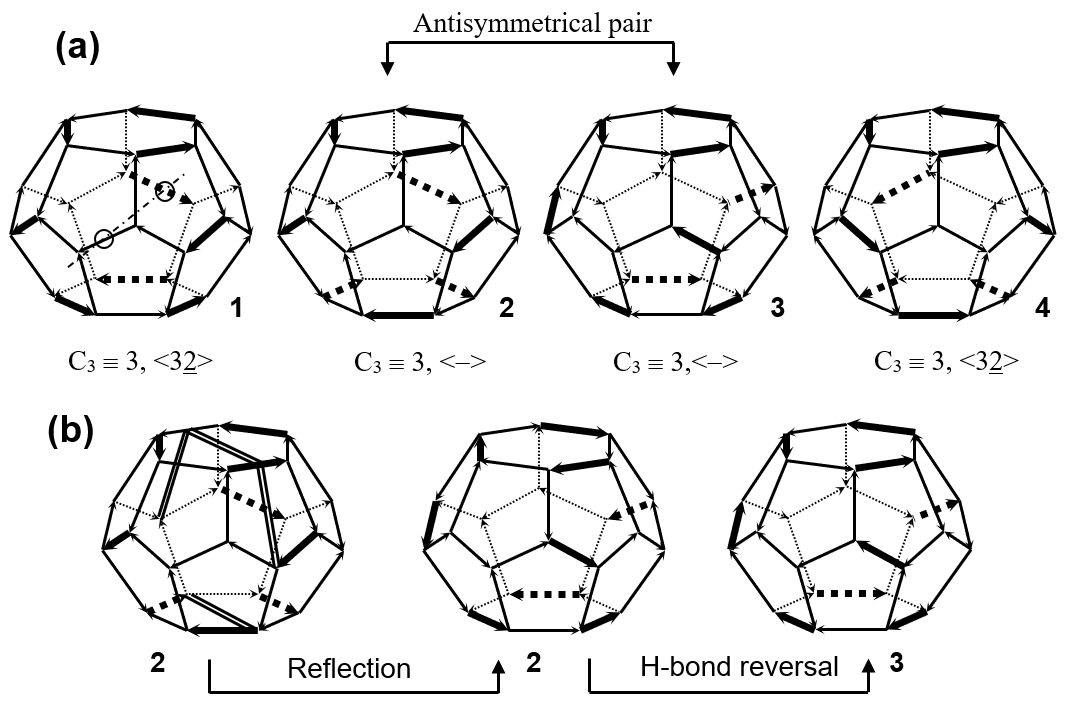
\includegraphics[width=.9\textwidth]{Figures/Chapter_6/symmetry_operations.png}
\end{center}
\begin{spacing}{1.0}
\caption[(a) Four lowest energy configurations of \ce{(H2O)_{24}} polyhedron. The arrows indicate the direction of the hydrogen bond: from the proton donor to the acceptor. In configurations 1 and 4, the lateral antisymmetry axes 2 (circles) pass through one t1d-bond that are shown with bold lines. (b) The antisymmetry transformation (anti-reflection in plane) which relates antipode configurations 2 and 3. This emphasizes the connection between near-symmetry and low-energy configurations.]{(a) Four lowest energy configurations of \ce{(H2O)_{24}} polyhedron. The arrows indicate the direction of the hydrogen bond: from the proton donor to the acceptor. In configurations 1 and 4, the lateral antisymmetry axes 2 (circles) pass through one t1d-bond that are shown with bold lines. (b) The antisymmetry transformation (anti-reflection in plane) which relates antipode configurations 2 and 3. This emphasizes the connection between near-symmetry and low-energy configurations.}\label{fig:MBE_III_F7}
\end{spacing}
\end{figure}